\documentclass{article}
\usepackage{amsfonts}
\usepackage{amsmath}
\usepackage{amsthm}
\usepackage{algorithm}
\usepackage{algorithmic}
\usepackage{bm}
\usepackage{hyperref}
\usepackage{footmisc}
\usepackage{xcolor}
\DeclareMathOperator\E{\mathbb{E}}
\DeclareMathOperator\Var{\mathrm{Var}}
\def\R{\mathbb{R}}
\def\P{\mathcal{P}}
\usepackage{mathtools}
\DeclarePairedDelimiter\abs{\lvert}{\rvert}
\DeclarePairedDelimiter\norm{\lVert}{\rVert}
\DeclarePairedDelimiter\inner{\langle}{\rangle}
\def\red#1{\textcolor{red}{#1}}
\makeatletter
\newcommand{\algorithmicfunction}{\textbf{function}}
\newcommand{\algorithmicendfunction}{\algorithmicend\ \algorithmicfunction}
\newenvironment{ALC@func}{\begin{ALC@g}}{\end{ALC@g}}
\newcommand{\FUNCTION}[2][default]{\ALC@it\algorithmicfunction\ #2\ %
\textbf{:}%
\ALC@com{#1}\begin{ALC@func}}
\ifthenelse{\boolean{ALC@noend}}{
    \newcommand{\ENDFUNCTION}{\end{ALC@func}}
  }{
    \newcommand{\ENDFUNCTION}{\end{ALC@func}\ALC@it\algorithmicendfunction}
  }
\makeatother
\theoremstyle{definition}
\newtheorem{definition}{Definition}
\newtheorem{theorem}{Theorem}
\newtheorem{example}{Example}
\newtheorem{corollary}{Corollary}
\newtheorem{lemma}{Lemma}
\newtheorem{remark}{Remark}
\begin{document}
If the graph weights are similar, we cannot distinguish each cluster. 
In such case, info-clustering algorithm will provide trivial solution: 
that is, either the whole set is one cluster or each singleton forms one cluster.

We consider one extreme case where the graph is complete graph and each edge is \textbf{with equal weight value} (suppose equal to 1 for brevity).
Then we will show that the info-clustering \textbf{solution is trivial}.

Recall that $f[\P] = \frac{1}{2}\sum_{C\in\P} f(C)$ where $f(C)$ is cut function.
\begin{lemma}\label{lem:L}
\begin{equation}\label{eq:larger_n_2}
\frac{f[\P]}{\abs{\P}-1} \geq \frac{n}{2}, \quad\forall \P
\end{equation}
where $n = \abs{V}$ and the equality holds only when $\abs{\P}=n$.
\end{lemma}
\begin{proof}
Math deduction on $\abs{\P}$ to prove $f[\P] \geq \frac{n}{2}(\abs{\P} - 1)$.  We know that the equality holds for $\abs{\P} = n$.
Suppose \eqref{eq:larger_n_2} holds for $\abs{\P} =k+1$. For $\abs{\P}=k(k\geq 2)$, the new paritition $\widetilde{\P}$ can be divided into $n_1\leq n_2 \dots n_k$ parts where $n_1 \leq \frac{n}{k}$.

Let the smallest part be further partitioned into two parts with $1$ and $n_1-1$ elements respectively.
Then using assumption that that the conclusion holds for $\abs{\P}=k+1$ we have
$$
n-1 + (n_1-1)(n-n_1+1) + \sum_{i=2}^k n_i(n-n_i) \geq nk
$$
That is $\sum_{i=1}^k n_i(n-n_i) \geq nk - 2(n_1-1)$
Since $2(n_1-1)<2n_1\leq 2\frac{n}{k} \leq n$ we have
$$
 \sum_{i=1}^k n_i(n-n_i)  > n(k-1)
$$
That it, strict inequality holds for $\abs{\P}=k$.
\end{proof}
According to Dilworth truncation theory, the line $-\lambda$ and $\frac{n(n-1)}{2} - n\lambda$ intersects at $(\frac{n}{2}, -\frac{n}{2})$. The minimal value for $\sum_{C\in\P}f(C) -\abs{\P}\lambda$ at $\lambda = \frac{n}{2}$ is $-\frac{n}{2}$ from lemma \ref{lem:L}. Therefore, the partition is trival.

From agglomerative point of view, $I(Z_V) \geq I(Z_C)$ for $C\in V$ if $G(V, E)$ is a complete graph with equal weight since we merge the set with largest MMI together.

generally speaking for a graph with weight $w_{ij}$ the info-clustering solution is trival if and only if
\begin{equation}\label{eq:GF}
\frac{f[\P]}{\abs{\P}-1} \geq \frac{\sum w_{ij}}{n-1} \textrm{ for any } \P
\end{equation}
holds.

For example, consider a graph with three point, when 
\begin{align*}
w_{12}+w_{23}\geq & w_{13} \\
w_{13}+w_{12}\geq & w_{23} \\
w_{13}+w_{23}\geq & w_{12} 
\end{align*}
That is, $w_{12}, w_{23}, w_{13}$ can be used to form a triangle in Euclidean space. Then we cannot get non-trival solution.

The triangle condition can be formulated as a sufficient condition:
\begin{lemma}
If $w_{ij}, w_{jk}, w_{ki}$ can form a triangle(or forms a line) in Euclidean space for any $i, j, k$, then the info-clustering solution is trival.
\end{lemma}
\begin{proof}
We use deduction to show  \eqref{eq:GF} holds. For $\abs{\P}=n$, the result holds. Suppose the result holds for any $\abs{\P} \geq k+1(k\geq 2)$, and for $\abs{\P}=k$, we choose the smallest part $C_1$ with $\abs{C_1}=n_1(\geq 2)$ and divide it into singletons. Then we have $k+n_1-1$ part. Using the assumption we have
$$
\mathrm{LHS} = \sum_{i\in C_1, i\neq k} w_{ik} + \sum_{r=2}^k \sum_{i \in C_r, j \not\in C_r} w_{ij}\geq \frac{2(k+n_1 -1)\sum w_{ij}}{n-1}
$$

Then for the given $\abs{\P}=k$, $2f[\P] =\mathrm{LHS} - \sum_{i,j\in C_1, i\neq j} w_{ij}$.
Applying triangle inequality $w_{ij} \leq w_{ik} + w_{jk}$ for given $k\not\in C_1$ and sum it over all $i, j \in C_1, i\neq j$, we have
$$
\sum_{i,j \in C_1, i\neq j} w_{ij} \leq 2(n_1-1)\sum_{i\in C_1} w_{ik}
$$
Since
\begin{align*}
\sum w_{ij} &= \sum_{i,j \in C_1, i\neq j} w_{ij} + \sum_{i\in C_1, k\neq C_1} w_{ik} \\
(n - n_1) \sum_{i,j \in C_1, i\neq j} w_{ij}& \leq 2(n_1 - 1) \sum_{i \in C_1, k \not\in C_1} w_{ik} \\
\end{align*}
We have $\sum_{i,j \in C_1, i\neq j} w_{ij} \leq \frac{2(n_1-1) \sum w_{ij}}{n-1}$. Therefore, 
$2f[\P] \geq \frac{2k \sum w_{ij}}{n-1}$. That is, the result holds for $\abs{\P}=k$.
\end{proof}
If we can use $w_{ij}$ as length of edge and can draw the graph on the Euclidean space, then the info-clustering solution is trival.

The above lemma gives us the following proposition:
For example, suppose all $w_{ij} \in [2,4]$, then the solution is trival.

From the hierachical structure property, we can get the following proposition.

\begin{proposition}
If $G$ has a subgraph $S$ which only admits trival solution, then neither non-singleton proper subset of $S$ is a cluster of $G$. 
\end{proposition}

\begin{proof}
Suppose  $S$ has a non-singleton subset $T$ which is a cluster of $G$, since $S$ only admits trival solution. $I(Z_S) > I(Z_T)$ and $S$ is also a cluster of $G$. In the hierachical tree of $G$, $S$ will be parent of $T$, from the top-down interpretation it is impossible since the clustering solution of $S$ is trival.
\end{proof}
\begin{example}\label{ex:6point}
\begin{figure}[!ht]
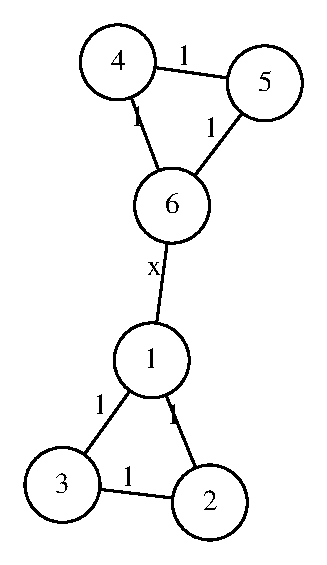
\includegraphics[width=6cm]{pic/6point.eps}
\end{figure}
In this example, $V=\{1,2,3,4,5,6\}$ and we have $I(Z_{\{1,2,3\}})=\frac{3}{2}, I(Z_V) = \min\{x,\frac{x+6}{5}, \frac{3}{2}\}, I(Z_{\{1,6\}})=x$, Then
\begin{equation*}
C^*(Z_V) = 
\begin{cases}
\{\{1,2,3\},\{4,5,6\}\} & x < \frac{3}{2} \\
\emptyset & x = \frac{3}{2} \\
\{1,6\} & x>\frac{3}{2}
\end{cases}
\end{equation*}
Where $C^*(Z_V)$ denotes the non-trival cluster of $V$.
\end{example}
\begin{proposition}\label{prop:sub}
If node set $S_1 \cap S_2 \neq \emptyset$ and $I(Z_{S_1}) > I(Z_{S_2})$, then $S_2$ is not a cluster of $G$.
\end{proposition}
\begin{proof}
Since $I(Z_{S_1\cup S_2}) > \min\{I(Z_{S_1}), I(Z_{S_2})\} = I(Z_{S_2})$. Then from the definition of info-cluster $S_2$ cannot be a cluster of $G$.
Since every two clusters of $G$ are either disjoint or have the inclusion relationship, $S_2$ cannot be a cluster of $G$.
\end{proof}
\begin{example}\label{ex:2c}
We extend example \ref{ex:6point}. Consider two complete graphs $S_1, S_2$ with $n$ nodes (weight = 1), there are $m$ connections(edges) between the two complete graphs, but all inter-connection edge is with equal weight 1. Also, suppose there is no complete graph with $n+1$ nodes in the $2n$-nodes graph. Since $I(Z_{S_1})=\frac{n}{2}$ which is largest among all subgraphs with no more than $n$ nodes and equal weight 1(since the solution to $S_1$ is trival). Therefore $I(Z_V) = \min\{m, \frac{m+n(n-1)}{2n-1}\}$. By some deduction, we get
\begin{equation*}
I(Z_V) = \begin{cases}
m & m <\frac{n}{2}, S_1,S_2 \textrm{ are non-trival cluster} \\
\frac{m+n(n-1)}{2n-1} & m\geq \frac{n}{2}, \textrm{ only trival solution} 
\end{cases}
\end{equation*}
In general, if we have $k$ clusters with each cluster a $n-$ clique. There are $m$ connections(edges) between any two different cliques. 
We have
\begin{equation*}
I(Z_V) = \begin{cases}
\frac{m}{k-1} & m <\frac{n(k-1)}{2}, S_i,\dots, S_k \textrm{ are non-trival cluster} \\
\frac{m+n(n-1)k/2}{kn-1} & m\geq \frac{n(k-1)}{2}, \textrm{ only trival solution} 
\end{cases}
\end{equation*}
\end{example}
\begin{example}
We make an improvement to example \ref{ex:2c}.
Suppose $S_1, S_2 $ are complete graph with $n$ nodes and equal weight $r=n$. Then $I(Z_{S_1})= \frac{nr}{2}$. there are $m$ connections(edges) between the two complete graphs, but all inter-connection edge is with equal weight 1. Then for any $U \in S_1 \cup S_2 $ and $\abs{U} < n$ by proposition \ref{prop:sub} we can show $U$ is not a cluster.
For $\abs{U} > n$ but $U \neq V = S_1 \cup S_2$. $I_{Z_U}$ can only be reached by $\{\{i\}| i\in U\}$, which is $\frac{\frac{n(n-1)r}{2} + m + \frac{k(k-1)r}{2}}{n+k-1}$ where $m \leq nk$ and $k=\abs{U} - n < n$. We compare it to $\frac{nr}{2}$ and we can show that $I(Z_{S_1}) \geq I(Z_U) $, that is $U$ is not a cluster by propsition \ref{prop:sub}. 
In such case, we call the graph $S_1$ is robust enough since complete linkage between the two clusters cannot destroy its structure. And we can get
\begin{equation*}
I(Z_V) = \begin{cases}
m & m <\frac{n^2}{2}, S_1,S_2 \textrm{ are non-trival cluster} \\
\frac{m+n(n-1)}{2n-1} & m\geq \frac{n^2}{2}, \textrm{ only trival solution} 
\end{cases}
\end{equation*}
This example inspires us to assign the weight value to unweighted graph as the number of triangle (3 node cliques) the edges contribute plus 1. In such case $ r = n-1$ and suboptimal result can be obtained. 
\end{example}
\end{document}